\documentclass[conference]{IEEEtran} 
\usepackage[utf8x]{inputenc}
\usepackage{graphicx}
\graphicspath{ {images/} }

\IEEEoverridecommandlockouts

\begin{document}

\title{\LARGE \bf Image classificiation and convolutional neural networks}

\author{\IEEEauthorblockN{Dawid Bitner, Daniel Broczkowski, Mateusz Kowol, Marcin Krupa}
\IEEEauthorblockA{Silesian University of Technology,\\
Faculty of Applied Mathematics}}



\maketitle
\thispagestyle{empty}
\pagestyle{empty}


%%%%%%%%%%%%%%%%%%%%%%%%%%%%%%%%%%%%%%%%%%%%%%%%%%%%%%%%%%%%%%%%%%%%%%%%%%%%%%%%
\begin{abstract}
Image classification - we define it as a task of extracting information classes from a multiband raster image. Its objective is to identify and portray, as a unique gray or color level, features occurring in an image in terms of the object or type of land cover these features represent on the ground, followed by grouping of all or selected land cover features into summary categories.

Combined with powerful Convolutional Networks (CNN), which are perfect for classification tasks, like image classification or processing natural language, we can create a great tool for classification purposes, in this case image classification. The main advantage of CNN compared to its predecessors is that it automatically detects the important features without any human supervision, as well as it is computationally efficient compared to other classification algorithms.

This article purpose is to bring the closer look to Convolutional Network and image classification in general.
\end{abstract}


%%%%%%%%%%%%%%%%%%%%%%%%%%%%%%%%%%%%%%%%%%%%%%%%%%%%%%%%%%%%%%%%%%%%%%%%%%%%%%%%
\section{INTRODUCTION}
\subsection{Terms related with image analysis}
Image analysis is simply a process of extracting meaningful information by computers to recognize attributes within an image. The means used to do so are mostly image processing techniques. Image analysis tasks can be very simple: reading bar coded tags or as sophisticated as identifying a person from their face. There are terms closely related with image analysis, worth explaining:
\\
\subsubsection{Computer vision}
CV, an abbrevation of Computer Vision, is defined as a field of study that works on enabling computers to see, identify and process content of digital images such as photographs and videos in the same way that human vision does, providing appropriate output.

Because computer must interpret what it sees, then perform appropriate analysis, we commonly link it with any type of artificial intelligence, as it is constantly processing and providing useful results based on the observation.
\\
\subsubsection{Image recognition}
Image recognition is a term for computer technologies that can recognize targets such as people, animals, objects etc. through the use of algorithms and machine learning. It can be done in many different ways, but most of them involves the use of convolutional neural networks, which will be described later, for now most important information is that it was specifically set up for image recognition and similar image processing.

Using characteristic techniques for CNN such as max pooling, stride configuration and padding, convolutional neural filters work on images to help machine learning programs get better at identifying the subject of the picture.
\\
\subsubsection{Image classification}
Image classification refers to the task of extracting information classes from a multiband raster image. This process categorizes all pixels in a digital image into one of several land cover classes, commonly refered as "themes". This categorized data may then be used to produce thematic maps of the land cover present in an image. There are two types of classification: supervised and unsupervised.

Supervised classification helps us identify examples of the information classes (i.e., land cover type) of interest in the image. These are called "training sites". It uses the spectral signatures obtained from training samples to classify an image.

The unsupervised classification examines a large number of unknown pixels and divides into a number of classed based on natural groupings present in the image values. It finds spectral classes (or clusters) in a multiband image without the analyst’s intervention.
\\
\subsubsection{Image processing}
Image processing converts an image into digital form to make operations on it, in order to get an enhanced image or to extract some useful information from it. It is a type of signal dispensation in which input is image, it can be a video frame or photograph and as an output may be image or characteristics associated with that image. It includes treating images as two dimensional signals while applying already set signal processing methods to them. 
\subsection{Convolutional Neural Network}
A Convolutional Neural Network (ConvNet/CNN) is a Deep Learning algorithm which can take image as an input and by a list of layers transform the image volume into an output volume. It can assign importance (learnable weights and biases) to various aspects/objects in the image and be able to differentiate one from the other. It's strong point is that pre-processing in a ConvNet does not requre that much computing power compared to other classification algorithms. While in primitive methods filters are hand-engineered, with enough training, ConvNets have the ability to learn these filters/characteristics. More about Convolutional Neural Network will be described in math section.
\subsection{Why and where do we use it?}
Image classification is enormously popular nowadays. This technology can be used in many different kind of domains like Website databases, city monitoring or intelligent cars such as popular "Testla".

If a visual database does not contain metadata about the images, categorizing it is a huge hassle. Classification of images through machine learning is a key solution for it. With image recognition, companies can easily organize and categorize their database because it allows for automatic classification of images in large quantities. This helps them monetize their visual content without investing countless hours for manual sorting and tagging.

The most recent and complicated application is used in China. Mass surveillance is the complicated network of surveillance used by the Chinese government to supervise the actions of Chinese citizens. In China, mass surveillance mainly comes from the government, though non-publicized corporate surveillance is also a possibility. There are multiple ways in which the Chinese state engages in surveillance, including Internet surveillance, camera surveillance in public, social credit surveillance, and other supporting digital technologies. Chinese mass surveillance has witnessed an increased spending, intensity, and coverage in recent years.

Another example may be very simplistic. Cars fitted with computer vision, that are able to perfectly classify, identify and distinguish objects on and around the road such as traffic lights, pedestrians, traffic signs and so on,  to act accordingly. The intelligent device could provide inputs to the driver or even make the car stop if there is a sudden obstacle on the road that is classified as something dangerous.

These are just some of them and it is hard to count them all. We are heading to the moment in the history when Artificial Intelligence is not just a fantasy, but it has a real impact on basically every aspect of our lives.
\\
\section{MATHEMATICAL DESCRIPTION}
This section will mainly focus on Convolutional Neural Network, as it is a main brain and source of power of anyimage classification systems.
\subsection{What are the ConvNets?}
Convolutional Neural Network is an architecture of neural network that is great at detecting and hierarchical learning of features, i.e. which features are worth attention and how to process them without human supervision. Usually we present it as list of layers that transform the image volume into an output volume (e.g. holding the class scores). To some extent they are similar in construction to ordinary neural networks, but the significant difference is that ConvNet networks have been designed to process images and objects that are on them. Thanks to the use of appropriate filters, it is easier for them to capture spatial dependencies on the image. Each layer accepts an input 3D volume and transforms it to an output 3D volume through a differentiable function, as well as they may have additional hyperparameters or not. The pre-processing required in ConvNet networks is much lower compared to other classification algorithms. The architecture provides a better match to the set of data consisting of images by reducing the number of parameters involved and the reusability of weights, making the forward function  more efficient in implementation.

The ConvNet network architecture consists of several layers that transform the original image layer by layer to the values needed to classify, such as:
\begin{itemize}
    \item input layer
    \item convolution layers
    \item activation layers
    \item pooling layers
    \item fully-connected layers
\end{itemize}
\subsection{Input layer}
In the ConvNet network, where we give an image to the input, the neurons are arranged in three dimensions: width, height and depth. Neurons in the layer will only be connected to the small area of the previous layer instead of the full connection. The output layer will reduce the full image to a single classification vector, located along the depth dimension. It is important to reduce images to a form that is easier to process, without losing the features that are key to getting a good result. It is important that our architecture should scale to huge data sets.

\begin{figure}[hbt!]
 \centering
    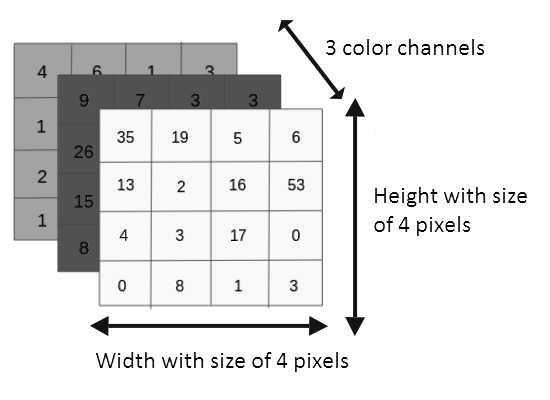
\includegraphics[scale=0.5]{input_layer-b.png}
	    \caption{Example of an input in form of an image in ConvNet}
	    \label{fig:my_label}
\end{figure}

\subsection{Convolutional layers}
Main block of the CNN network. They contain a set of filters that are learnable. Convolution is a mathematical operation to merge two functions, creating a new third. In case of a network where an image is input, the convolution is used on the input data by the convolutional filter (kernel) to create a feature map.
We perform the convolution operation by sliding this filter over the input. Matrix multiplication is performed and the sum is written on the feature map.

\begin{figure}[hbt!]
 \centering
    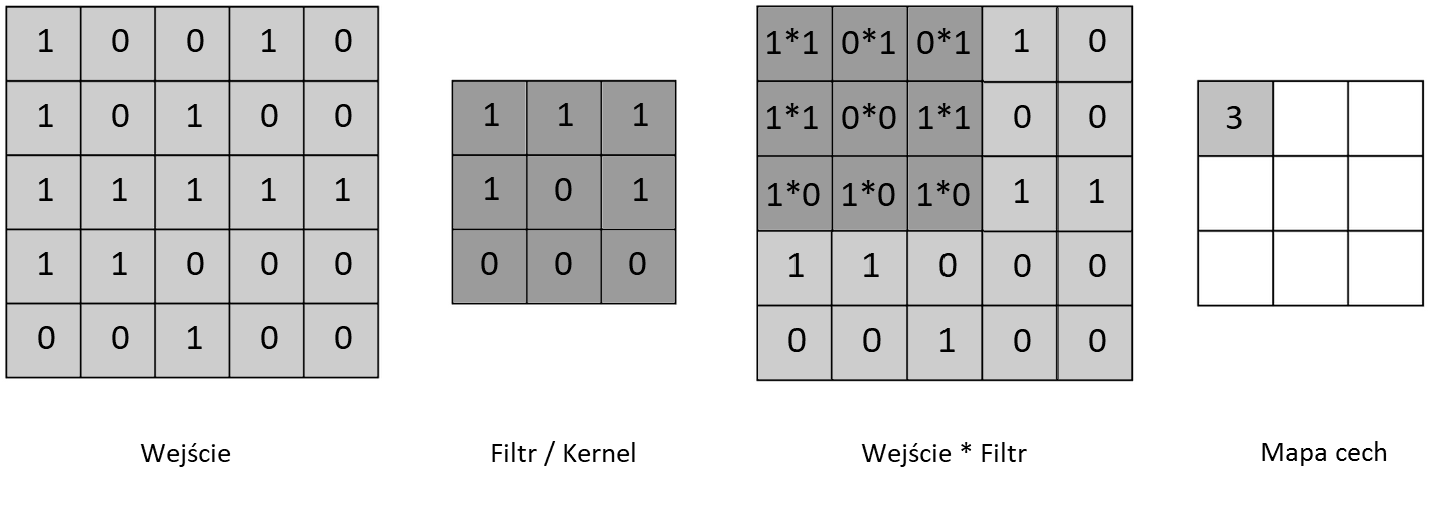
\includegraphics[scale=0.24]{kernel-b.png}
	    \caption{Example use of 3x3 filter on two dimensional input data. Kernel moves on top of the input, and the sum of the operation goes to the feature map.}
	    \label{fig:my_label}
\end{figure}

The above example is made in 2D. But in ConvNet networks we performe convolutions on images, represented as a 3D matrix with three dimensions: height, width and depth, where the depth represents color channels. Kernel used over the image must also be 3D, as it covers the entire depth of the input.

Many convolutions are made over the imput, each using a different filter and resulting in a separate feature map. Later, the combination of all these feature maps becomes our final result of the convolutional layer.

Generally, the purpose of the convolution is to extract features such as edges from the input image. ConvNets do not have to be limited to only one layer of convolution. Traditionally, the first ConvLayer is responsible for capturing features such as edges, color, gradient descent etc., and by adding more layers, you can expand and tune the architecture. We can get a network that understands images similar to us.

\begin{figure}[hbt!]
 \centering
    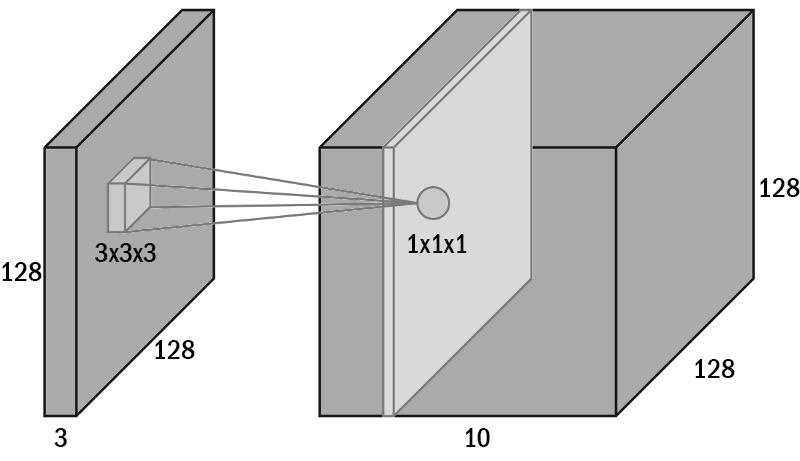
\includegraphics[scale=0.25]{3dkernel-b.png}
	    \caption{Example use of 3x3 filter on two dimensional input data. Kernel moves on top of the input, and the sum of the operation goes to the feature map.}
	    \label{fig:my_label}
\end{figure}

Example: above image shows a 128x128x3 image, the kernel has the size of 3x3x3. When the filter is over a specific location and covers a small volume of an input, we perform a convolution operation similar to the 2D example, except that this one takes place in three dimensions. As a result we still get a scalar. By sliding the filter over the input, we calculate the next values, and properly record them on the feature map of size 128x128x1. The size of width and heigh does not change due to the use of padding, as we use this technique to maintain the same dimensionality. In order to do that, we surround the input with zeros or values on the edges. What changes is the depth of an image, it is reduced to just one channel.

If we are using 10 different filters, we get 10 different maps of features with a size of 128x128x1. Putting them along the depth dimension would give us the final result of the convolutional layer: a volume of size 128x128x1. The convolution operation for each filter is done independently, and the resulting feature maps are disjoint.

\subsection{Activation layer}
ConvNe is no exception when it comes to using the activation function between layers. There are many functions to pass the result of the convolution operation. Most popular ones are ReLU and sigmoid functions. Using the activation function, we must keep in mind that the values in the final feature maps are not really sums, but the values after applying activation function to them, and that each type of convolution requires an activation function, without them the network will not reach its full potential.

ReLU formula:
$$R(z)=max(0, z)$$
$$z=Wx + b$$

Sigmoid formula:
$$\sigma\left(z\right)=\frac{1}{1+e^{-z}}$$

\begin{figure}[hbt!]
 \centering
    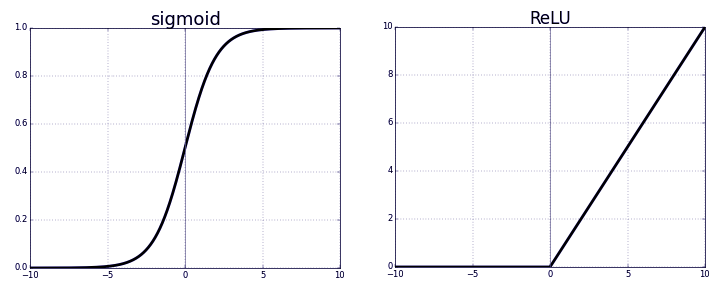
\includegraphics[scale=0.45]{act_graph.png}
	    \caption{Comparison of ReLU and sigmoid on the graph.}
	    \label{fig:my_label}
\end{figure}

ReLU is more common for ConvNets for several reasons: it has reduced gradient probability (change in the direction of intensity or color of the image), it is more computationally efficient for calculation than sigmoid functions (ReLU only needs to select $max(0, z)$ and does not perform costly exponential operations).

\subsection{Strides, max-pooling, padding}
Stride is a parameter that determines by how many values we are overlapping the convolution filter over an image at each step. We can decide on the value of it - if it is large, the resulting feature map is smaller because we are skipping the potential locations.

\begin{figure}[hbt!]
 \centering
    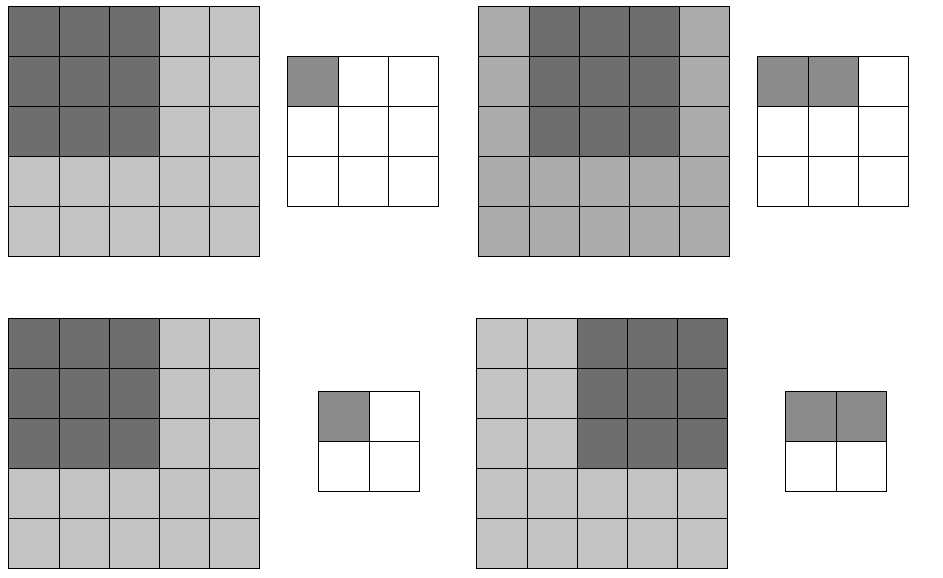
\includegraphics[scale=0.36]{stride_comparison-b.png}
	    \caption{Comparison of ReLU and sigmoid on the graph.}
	    \label{fig:my_label}
\end{figure}

Using strides we create a feature map that is smaller than the size of the of the input, because the convolution filter must be contained in the input data. If we want to maintain the same dimensionality, we can use padding to surround the input with zeros or values that are on the edge of an image. It is a common technique to keep the size of the feature maps to prevent shrinkage on each layer. Just like in the two dimensional picture, we use them on convolutional layers that are in 3D.

\begin{figure}[hbt!]
 \centering
    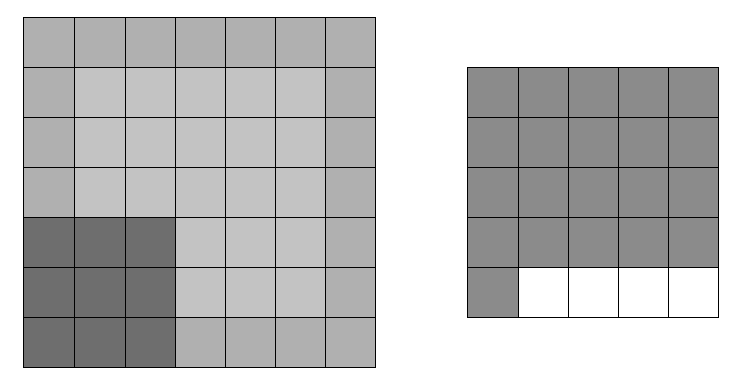
\includegraphics[scale=0.36]{padding-b.png}
	    \caption{Example of padding.}
	    \label{fig:my_label}
\end{figure}

Next is pooling that reduces "dimensionality" of an input, which is a convolutional layer, to lower the number of parameters. It shortens the training time and prevent from overfitting. If the network is large, this technique can reduce the number of weights between layers a lot. Height and width of the feature map are halved, but the depth does not change because pooling works independently on each depth slice the input.
Commonly we use max-pooling, which gets the maximum value in the "operation window". Max-pooling has no parameters, it is just an process of slidding this operation window over the input and getting the maximum value. The window size and stride are predefined. To generalize pooling layer:
\begin{itemize}
    \item Accepts a volume of size $W_{1}×H_{1}×D_{1}$
    \item Requires two hyperparameters:
    \begin{itemize}
        \item their spatial extent $F$,
        \item the stride $S$
    \end{itemize}
    \item It produces a volume of size $W_{2}×H_{2}×D_{2}$, where:
    \begin{itemize}
        \item $W_{2}=\frac{W_{1}F}{S} + 1$
        \item $H_{2}=\frac{H_{1}F}{S} + 1$
        \item $D_{2}=D_{1}$
    \end{itemize}
\end{itemize}
\begin{center}
    \begin{figure}[hbt!]
 \centering
    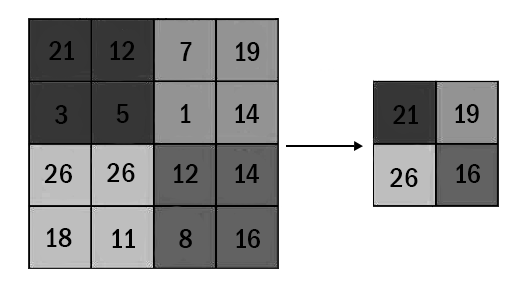
\includegraphics[scale=0.35]{maxpool-b.png}
	    \caption{Max-pooling.}
	    \label{fig:my_label}
\end{figure}
\end{center}

\subsection{Hyperparameters}
These are parameters that we should consider more wisely when creating a ConvNet network. They include:
\begin{itemize}
    \item Filter size - if it is small, more detailed information can be extracted from the image and reused later (it can also act on the contrary: completely useless information can be extracted), slows down decrease in size of an image. Larger filters isolate quite general features in the image, the amount of information extracted is much smaller. Fast image size reduction makes the network quite shallow.
    \item Number of filters - the most alternating parameter in CNN network, usually a value between 32 and 1024. Using more filters gives a more powerful model, but we risk overfitting due to the increased number of parameters. Usually we start with a small number of filters in the initial layers and gradually increase the number when we go deeper into the network.
    \item Stride and Padding
\end{itemize}
\subsection{Fully-connected layer}
After convolution and max-pooling, we add several fully-connected layers to complete the CNN architecture. These layers require 1D numbers for input, while convolution and pooling layers have a 3D vector. We must perform \textit{flattening}.

\begin{figure}[hbt!]
 \centering
    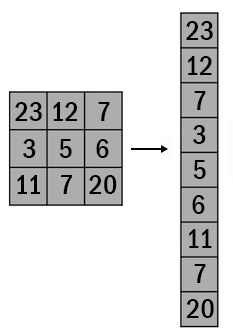
\includegraphics[scale=0.35]{flattening-b.png}
	    \caption{Flattening the input to a one dimensional vector.}
	    \label{fig:my_label}
\end{figure}

The flattened output signal is fed to the neural network, and as in the classical network, backward propagation applied to each iteration. After a series of eras, the model is able to distinguish between dominant and irrelevant features in images and classify them using the \textit{Softmax} classification technique, that converts numbers into probabilities that sums up to one. Softmax derives a vector that represents the probability distributions of the list of potential results.

Softmax:
$$P\left(y=j | \sigma(z)_{i}\right)=\frac{e^{z_{i}}}{\sum_{j=1}^{K}e^{z_{j}}}$$
$$\sigma = w_{0}x_{0} + w_{1}x_{1} + ... + w_{k}x_{k} = \sum_{i=0}^{K} = w^{T}x$$

\begin{figure}[hbt!]
 \centering
    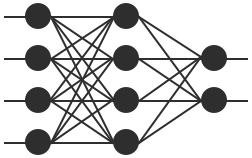
\includegraphics[scale=0.4]{fully_connected_network.png}
        \caption{Fully connected layer schema.}
	    \label{fig:my_label}
\end{figure}


To put fully-connected network in more mathematical way:
\begin{itemize}
    \item Let $x \in R_{m}$ represent the input to a fully connected layer.
    \item Let $x_{i} \in R_{m}$ be the $i$-th output from the fully connected layer.
\end{itemize}
Then $y_{i} \in R$ is computed as follows:
$$y_{i} = w_{1}x_{1} + ::: + w_{m}x_{m})$$
If we use ReLU activation function, and say $w$ and $i$ are learnable parameters in the network, the full output $y$ is as follows:
$$y = \sigma(w_{1,1}x_{1}+...+w_{1, m}x_{m})$$
\subsection{Dropouts}   
Dropout is used to prevent overfitting, that means we exclude neurons intentionally to prevent the network from being too dependent on a small number of neurons and forcing each neuron to act independently. Dropout is used on the input layers and hidden layers, but we do not use them on the output layer. During training in each iteration, the neuron is temporarily "dropped" or disabled with the probability \textit{p}. This means that all inputs and outputs to this neuron will be turned off at the current iteration. Abandoned neurons are re-sampled with the probability \textit{p} at each subsequent training step, so an dropped neuron in one step can be active in the next step. The hyperparameter \textit{p} is called the dropout-rate or a degree of decay and is usually about 0.5, which means that about $50\%$ of neurons are falling out.
\subsection{Loss function, cross-entropy}
Loss function is used to measure the inconsistency between predicted value $\left(\widehat{y}\right)$ and actual label $\left(y\right)$. It is a non-negative value, where the robustness of model increases along with the decrease of the value of loss function. Loss functions fall under four major category:
\begin{itemize}
    \item Regressive loss functions - used in case of regressive problems, that is when the target variable is continuous. Most widely used regressive loss function is Mean Square Error.
    $$MSE\left(\widehat{\theta}\right)= E\left(\left(\widehat{\theta}-\theta\right)^2\right)$$
    $\widehat{\theta}$ is an estimator of $\theta$.
    \item Classification loss functions - as an output in classification is a value f(x), called the score for the input x. The magnitude of the score represents the confidence of our prediction. The target variable y, is a binary variable, 1 for true and -1 for false.
    \item Embedding loss functions: - deals with problems where we have to measure whether two inputs are similar or dissimilar.
\end{itemize}

Cross-entropy is most common of all classification loss functions. It loss increases as the predicted probability diverges from the actual label. In information theory, the cross entropy between two probability
distributions $p$ and $q$ over the same underlying set of
events measures the average number of bits needed to identify
an event drawn from the set if a coding scheme used for the set
is optimized for an estimated probability distribution $q$, rather
than the true distribution $p$.
The cross entropy for the distributions $p$ and $q$ over a given set is defined as follows:
$$H(p,q)=E_{p}\left[-\log_{} q\right]$$

If we set up notation $p \in \{y, 1 - y\}$ and $q \in \{\widehat{y}, 1 - \widehat{y}\}$ we use cross entropy to measure dissimilarity between $p$ and $q$:
$$H(p,q)=-\sum_{i}\log_{}q_{i}=-y\log_{}\widehat{y}-\left(1-y\right)\log_{}\left(1-\widehat{y}\right)$$
The typical cost function that one uses in logistic regressionis computed by taking the average of all cross-entropies in the sample. For example, suppose we have $N$ samples with each sample indexed by $n=1,...,N$. The loss function is given by:
$$J\left(W\right)=-\frac{1}{N}\sum_{n=1}^{N}\left[y_{n}\log_{}\widehat{y}+\left(1-y_{n}\log_{}\left(1-\widehat{y}\right)\right)\right]$$
where $\widehat{y}=g\left(w\dot{x_{n}}=\frac{1}{1+e^{-w_{n}}}\right)$, $g(z)$ is the logistic function as before.

\subsection{Optlimazators}
During the network training process, we always adjust and change the parameters (weights) of our model to minimize the loss function and make our predictions as correct as possible. For this purpose, we use optimizers that update the model in response to the loss function result.

The classic example is gradient descent, used to decreased the cost function:
$$w_{n+1} = w_{n} - \eta \frac{\partial}{\partial w_{n}}J(w_{n})$$

But in ConvNets we use more sophisticated methods. One is Adaptive Moment Estimation (Adam). It computes adaptive learning rates for each parameter. In addition to storing an exponentially decaying average of past squared gradients $v_{t}$, it also keeps an exponentially decaying average of past gradients $m_{t}$. We compute the decaying averages of past and past squared gradients $m_{t}$ and $v_{t}$ using these formulas:

$$m_{t}=\beta_{1}m_{t-1}+\left(1-\beta_{1}\right)g_{t} \rightarrow mean$$
$$v_{t}=\beta_{2}m_{t-1}+\left(1-\beta_{2}\right)g_{t}^2 \rightarrow uncentered \: variance$$

$m_{t}$ and $v_{t}$ are estimates of the first moment (the mean) and the second moment (the uncentered variance) of the gradients. As $m_{t}$ and $v_{t}$ are initialized as vectors of 0's, they are biased towards zero, especially during the initial time steps, and especially when the decay rates are small (i.e. $\beta_{1}$ and $\beta_{2}$ are close to 1).

We counteract these biases by computing bias-corrected first and second moment estimates:

$$\widehat{m_{t}}=\frac{m_{t}}{1-\beta_{1}^t}$$
$$\widehat{v_{t}}=\frac{v_{t}}{1-\beta_{2}^t}$$

They then use these to update the parameters, which yields the Adam update rule:

$$\theta_{t+1}=\theta_{t}-\frac{\eta}{\sqrt{\widehat{v_{t}}}+\epsilon}\widehat{m_{t}}$$

Proposed default values are: 0.9 for $\beta_{1}$, 0.999 for $\beta_{2}$ and $10^{-8}$ for $\epsilon$.

\section{PROPOSED SYSTEM}
System that will be used for classification of 11 animals:

\begin{figure}[hbt!]
 \centering
    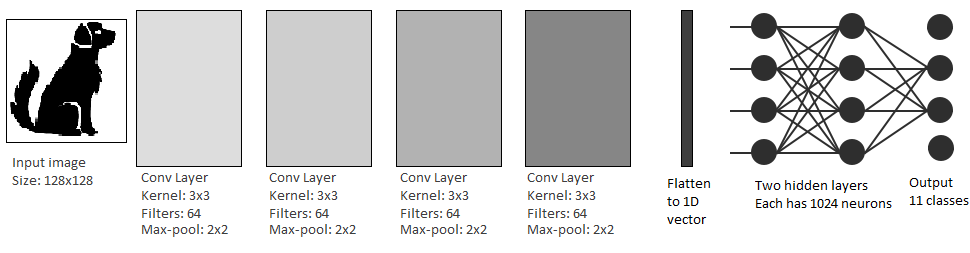
\includegraphics[scale=0.34]{convnet.png}
        \caption{Classification of animals step by step.}
	    \label{fig:my_label}
\end{figure}

\begin{enumerate}
    \item This setup is made of 4 convolutional layers in total. Each one has a ReLU activation function. Weights in filters are generated randomly and the have normal distribution with standard deviation of 0.05. Kernels/filters have a 3x3 size. Weight decay $0.001$. Each convolution layer has max-pooling next. Last layer, output one, uses Softmax activation function.
    \item As an optimizer we use Adam, as it is good at optimizing weights according to the loss
    function, which is cross-entropy. It's a very classic set.
    \item We have a dataset of 43.000 animals, belonging to 11 classes. The data was later splitted: $90\%$ of the dataset is used for training, $10\%$ for validation.
    \item Neural network is fed with batches of size containing 128 training images. During training it updates it weights. For validation it does not.
    \item Each step the training and validation loss are being printed, and every epoch ends with information how effective is the learning process.
    \item Describing it layer-by-layer:
    \begin{itemize}
        \item First layer: as an input takes 128x128x1 photo, so it has just one color channel, to make sure it is more computing efficient. The testing machine will be using graphic card for learning process.
        It applies convolution using 64 filters, creating an output of 128x128x64 for max-pooling layer. Later, the output of max-pooling layer is of size 64x64x64.
        \item Second layer: input - 64x64x64, after applying 128 filters the output is of size 64x64x128. Max-pooling creates an output of 32x32x128 for next layer.
        \item Third layer: input - 32x32x128, uses 128 filters output: 32x32x128, max-pooling: 16x16x128.
        \item Fourth layer: input - 16x16x128, uses 256 filters output: 16x16x256, max-pooling: 8x8x256.
        \item Flattening: 8x8x256 = 16384 input neurons.
        \item Two fully-connected hidden layers, each has 1024 neurons.
        \item Output layer, has 11 neurons, uses Softmax activation function.
    \end{itemize}
\end{enumerate}

\section{EXPERIMENTS}

As described earlier, the dataset consists of 43000 images of animals, that comes from different distributions. Images were taken in different light, the animals were turned in diffrenet direction (some images had to be flipped), but also the image themselves were of different quality. Because of such a vast imperfections in the dataset, zero-centering was used. It increased the accuracy by $2-3\%$.

\begin{figure}[hbt!]
 \centering
    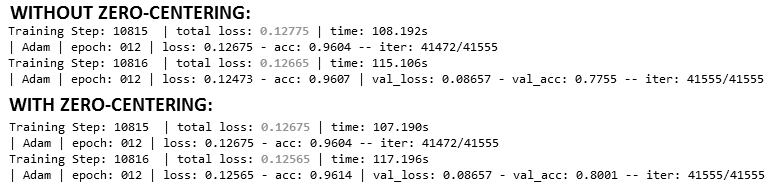
\includegraphics[scale=0.46]{adam_zc-b.png}
        \caption{With and without use of zero-centering, same amount of epochs.}
	    \label{fig:my_label}
\end{figure}

Experiments included changing filter number on every convolutional layer. If the number was small, it learned rapidly, but the results were far from good, no matter the number of epochs or batch size.
Network with more filters on each of convolutional layers, or with more convolutional layers started overfitting quite fast. This occurs when our model perform unusually well on its training data, but very poorly on new, unseen data. Model described earlier was just a decent balance.

More experiments were made creating a model with Adam as it's optimizer. $80\%$ was a maximum this network could get using Adam, and  it is a good practice to change later on Adam to something else, like Stochastic gradient descent (SGD) or RMSprop. Both were tested, both failed.

The reason SGD failed is because it is SGD. Meaning behind it is that SGD usually achieves to find a minimum, but it might take significantly longer than with some of the optimizers, it is much more reliant on a robust initialization and annealing schedule, and may get stuck in saddle points rather than local minima. It also takes much more time to get a decent results. That was the case.

\begin{figure}[hbt!]
 \centering
    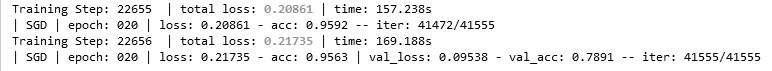
\includegraphics[scale=0.46]{sgd-b.png}
        \caption{Use of SGD. Accuracy drops down.}
	    \label{fig:my_label}
\end{figure}

Some of the graphs for a tested model:
\begin{figure}[hbt!]
 \centering
    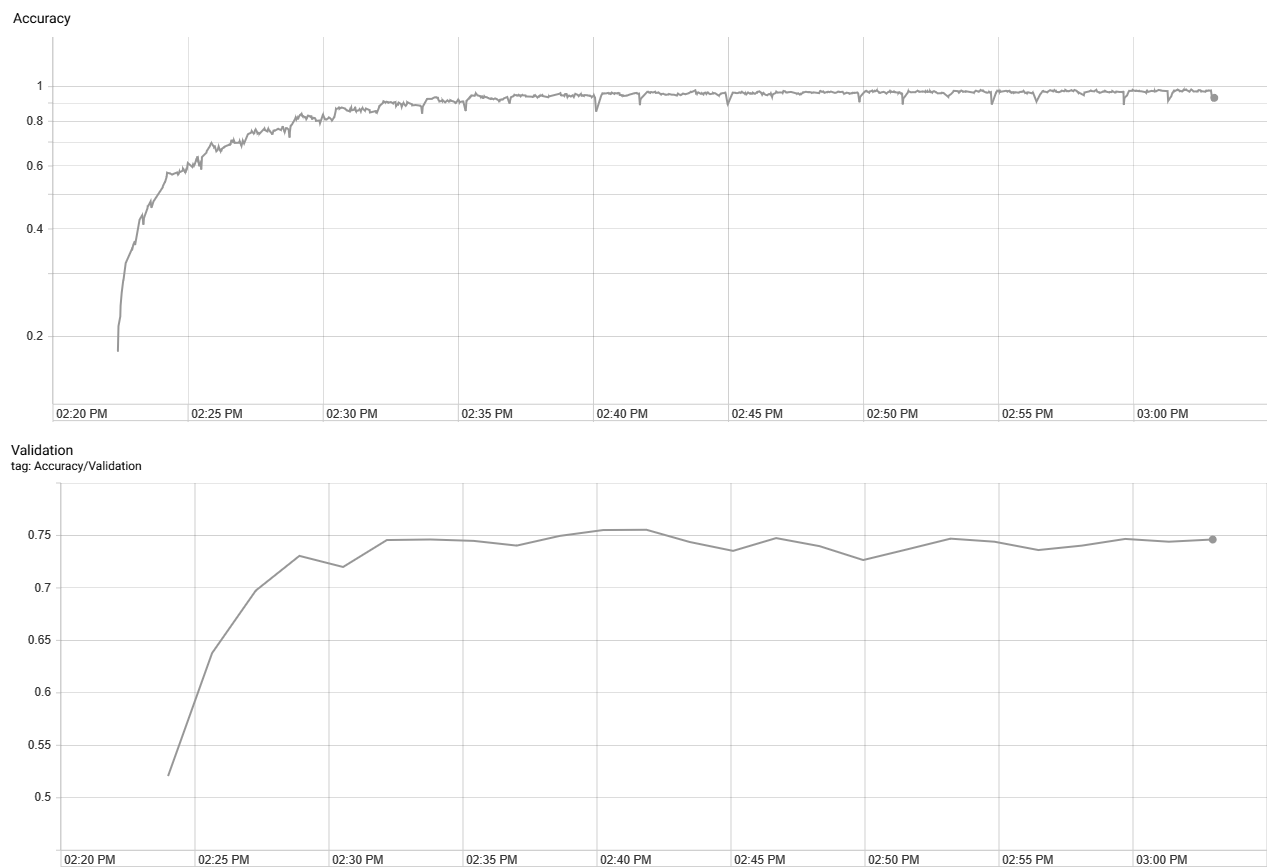
\includegraphics[scale=0.27]{accuracy.png}
        \caption{Graph shows the accuracy for training and validation data.}
	    \label{fig:my_label}
\end{figure}
\begin{figure}[hbt!]
 \centering
    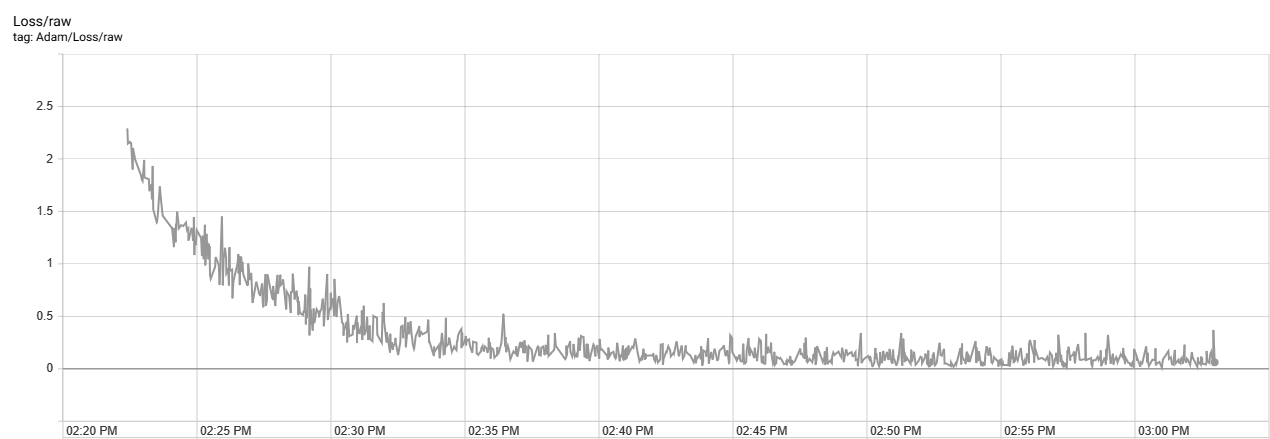
\includegraphics[scale=0.27]{adam_loss.png}
        \caption{Graph shows the Adam optimizer loss.}
	    \label{fig:my_label}
\end{figure}
\begin{figure}[hbt!]
 \centering
    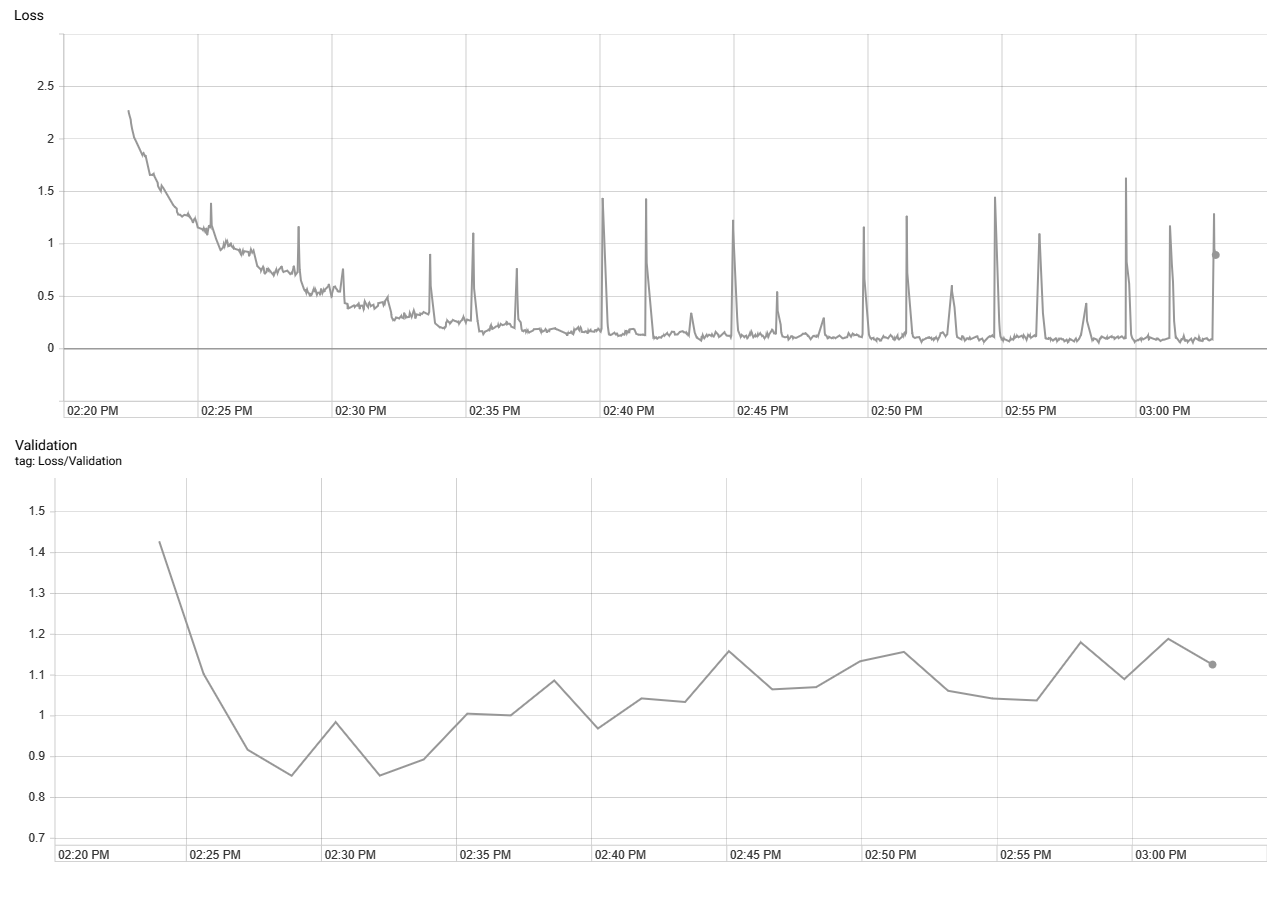
\includegraphics[scale=0.27]{loss.png}
        \caption{Graph shows the loss on training and validation data.}
	    \label{fig:my_label}
\end{figure}
\section{CONCLUSIONS}
Not perfect, but a very decent model created with around $78-80\%$ of accuracy. Even with the output size of 8x8x256 at the last convolutional layer after max-pooling, it did great at extracting essential features from an image, proving that convolutional neural network are a powerful tool for image classification.

Dataset consist of 43000 images, almost 4000 image per class. Network recognizes very well images that are similar to stock photos, and do very well with images that have clear contour of animal silhouette.  Otherwise, it classifies wrong.

How to improve this network? Firstly, using 3 color channels in the input image instead of just one grayscale. Color at natural image processing is very important, but it takes more computing power that the testing machine did not have. Secondly, improving the database to be  more vast at covering differences between the animals. Lastly, just spending more time on tuning the network by adjusting the kernel size, increasing number of layers and number of filters, giving more time to SGD to prove itself etc.

\section{BIBLIOGRAPHY}
\begin{itemize}
    \item Dertat A., \textit{Applied Deep Learning - Part 4: Convolutional Neural Networks}, https://towardsdatascience.com/applied-deep-learning-part-4-convolutional-neural-networks-584bc134c1e2, 2019-06-06
    \item Karpathy A., \textit{CS231n Convolutional Neural Networks for Visual Recognition}, http://cs231n.github.io/convolutional-networks/,  2019-06-06
    \item \textit{Overfitting in Machine Learning: What It Is and How to Prevent It}, https://elitedatascience.com/overfitting-in-machine-learning, 2019-06-06
    \item Reppel E., \textit{Visualizing parts of Convolutional Neural Networks using Keras and Cats}, https://hackernoon.com/visualizing-parts-of-convolutional-neural-networks-using-keras-and-cats-5cc01b214e59, 2019-06-06 
    \item Ruder S., \textit{An overview of gradient descent optimization algorithms}, http://ruder.io/optimizing-gradient-descent/index.html, 2019-06-06
    \item Saha S., \textit{A Comprehensive Guide to Convolutional Neural Networks - the ELI5 way}, https://towardsdatascience.com/a-comprehensive-guide-to-convolutional-neural-networks-the-eli5-way-3bd2b1164a53, 2019-06-06   
    \item Sahoo S., \textit{Deciding optimal kernel size for CNN}, https://towardsdatascience.com/deciding-optimal-filter-size-for-cnns-d6f7b56f9363, 2019-06-06  
    \item \textit{Supervised Learning}, https://www.techopedia.com/
    definition/30389/supervised-learning, 2019-06-06    
\end{itemize}
\end{document}
